% Viva / video slides. IIIT-H dark Beamer theme (Srikar Sharma Sadhu, GPL-3), files in this folder.
% Build: pdflatex slides && pdflatex slides
% Figures: PYTHONPATH=src python reports/slides/make_slide_figures.py (from the repository root)
\documentclass{beamer}
\usepackage{amsfonts,amsmath}
\usepackage{booktabs,array}
\usepackage{tikz}
\usetikzlibrary{positioning,arrows.meta,fit}
\usetheme{_statale}
\usefonttheme[onlymath]{serif}
\titlebackground*{assets/background}
\AtBeginSection[]{} % no table-of-contents slide at each section
\graphicspath{{figures/}}

\newcommand{\acn}[1]{\texttt{#1}}

\title{When Does Graph Expansion Help?}
\subtitle{Issue-adaptive retrieval routing for repository-level code localization}
\course{Information Retrieval and Extraction}
\author{Naman Singhal (2024114013)\newline Yash More (2024114004)\newline Aaditya Bhatia (2023114012)}
\date{November 2026}
\footlinepayoff{Singhal, More, Bhatia\enspace$\vert$\enspace When Does Graph Expansion Help?}

\begin{document}
\maketitle

% ============================================================
\section{Motivation}

\begin{frame}{The problem: finding the code to fix}
  \begin{itemize}
    \item Before a coding agent can fix an issue, it has to \textbf{find the relevant code}.
    \item It works under a \textbf{budget}: its context window is finite, so every chunk of code it reads pushes another one out.
    \item \textbf{Keyword (BM25) and embedding search} are cheap, but they miss code that shares no words with the issue and is linked to it only through calls, imports or inheritance.
    \item \textbf{Graph-based agents} (LocAgent, CoSIL, OrcaLoca) follow those links. But the choice of \emph{when} to follow them is hidden inside the LLM's reasoning.
  \end{itemize}
\end{frame}

\begin{frame}{Our question}
  \begin{block}{When does graph expansion help? Can we predict it in advance?}
  \end{block}
  \vspace{4pt}
  We expected the answer to depend on the issue:
  \begin{itemize}
    \item A pasted \textbf{traceback} names a function, so following its \textbf{calls} should help.
    \item An issue that \textbf{names the file} is already found by keyword search, so expanding only adds noise.
    \item If the top hit is a \textbf{hub}, its neighbours could flood the budget.
  \end{itemize}
  \vspace{4pt}
  \textbf{Phase A:} measure what each retrieval action is worth, issue by issue.\\
  \textbf{Phase B:} turn that into a router that picks one action per issue.
\end{frame}

% ============================================================
\section{Setup}

\begin{frame}{Overview}
  \centering
  \begin{tikzpicture}[
    node distance=0.35cm and 0.3cm,
    box/.style={draw=maincolor, rounded corners=2pt, align=center, font=\scriptsize,
                minimum height=0.75cm, inner sep=3pt, text=maincolor},
    act/.style={box, font=\scriptsize\ttfamily, minimum width=2.25cm, minimum height=0.36cm, inner sep=1.5pt},
    arr/.style={-{Latex[length=1.6mm]}, thick, draw=maincolor}
  ]
    \node[box] (issue) {Issue\\text};
    \node[box, right=of issue] (bm25) {BM25\\seed};
    \node[box, right=of bm25] (feat) {Post-seed\\features};
    \node[box, right=of feat, fill=frmtxt, text=toctxt, font=\scriptsize\bfseries] (router) {Router};
    \node[act, right=0.8cm of router, yshift=1.0cm] (a1) {stop};
    \node[act, below=0.04cm of a1] (a2) {dense};
    \node[act, below=0.04cm of a2] (a3) {fusion};
    \node[act, below=0.04cm of a3] (a4) {expand(calls)};
    \node[act, below=0.04cm of a4] (a5) {expand(imports)};
    \node[act, below=0.04cm of a5] (a6) {expand(inherit)};
    \node[draw=maincolor, dashed, rounded corners=3pt, fit=(a1)(a6), inner sep=3pt] (acts) {};
    \node[box, right=0.6cm of acts] (out) {Ranked\\chunks,\\cut to\\$B$ lines};
    \draw[arr] (issue) -- (bm25);
    \draw[arr] (bm25) -- (feat);
    \draw[arr] (feat) -- (router);
    \draw[arr] (router) -- (acts.west |- router);
    \draw[arr] (acts) -- (out);
  \end{tikzpicture}
  \vspace{6pt}
  \begin{itemize}
    \item \textbf{Phase A:} run all six actions on every issue, record each gain over the seed.
    \item \textbf{Phase B:} pick one action per issue in advance, from cheap features.
  \end{itemize}
\end{frame}

\begin{frame}{Data, budget and splits}
  \begin{itemize}
    \item \textbf{SWE-Explore} benchmark: the ground truth is the code that successful agents \emph{read} while fixing each issue.
    \item Its Python subset: \textbf{500 issues} (410 from SWE-bench Verified, 90 from SWE-bench Pro) from \textbf{15 repositories}. Django alone is 41\%.
    \item Every system returns ranked code chunks cut to a budget of \textbf{300 lines} (also 100 and 500).
    \item The ground truth is mostly \textbf{whole files} (median 1,160 lines), so even a perfect ranker reaches only 39.5\% recall at 300 lines.
    \item \textbf{Splits:} 56 dev issues (xarray, pytest, openlibrary) are used only for tuning. The other 444 form 8 \textbf{one-repository-held-out} folds.
  \end{itemize}
\end{frame}

\begin{frame}{Six retrieval actions}
  \begin{itemize}
    \item \acn{stop}: keep the BM25 seed.
    \item \acn{dense}: a frozen code embedding model (CodeRankEmbed, 137M parameters).
    \item \acn{fusion}: merge the BM25 and dense rankings (reciprocal-rank fusion, $k=100$ tuned on dev).
    \item \acn{expand(e)}: neighbours of the top 10 seed chunks along edge type $e$ (calls, imports, inheritance) move up the ranking:
      \[ s_e(n) = \max\big(s(n),\ \lambda \max_{p} s(p)\big) \]
    \item Tuned on dev: $\lambda = 0.99$ and edges followed in both directions, so a hit's callers and callees go right after it.
    \item Code graph: LocAgent's builder, adapted to run about \textbf{5 times faster} with the same edges.
  \end{itemize}
\end{frame}

\begin{frame}{Scoring: two problems in the benchmark}
  \begin{itemize}
    \item \textbf{Lines that do not exist.} Agents often ran \texttt{sed -n 1,240p} on shorter files. The benchmark keeps the requested range, so the official recall counts phantom lines. We clip ranges to the file.
    \item \textbf{nDCG that rewards one early hit.} The SWE-Explore paper builds nDCG's ideal ranking from the ground truth. The released code builds it from the system's own output.
    \item With the released code, \textbf{75 of the 500 BM25 seeds score a perfect 1.0} while covering only 14\% of the right code.
    \item We use the paper's definition as our main metric (it tracks recall better: correlation 0.55 against 0.42) and report both.
  \end{itemize}
\end{frame}

% ============================================================
\section{Phase A}

\begin{frame}{Phase A: on average, little changes}
  \centering
  \begin{tabular}{lccc}
    \toprule
    Action & nDCG@100 & nDCG@300 & nDCG@500 \\
    \midrule
    \acn{stop} (BM25 seed) & .264 & .172 & .144 \\
    \acn{expand(inherit)} & .264 & .172 & .144 \\
    \acn{expand(imports)} & .263 & .170 & .143 \\
    \acn{expand(calls)} & \textbf{.280} & .178 & .146 \\
    \acn{dense} & .213 & .152 & .128 \\
    \acn{fusion} & .268 & \textbf{.184} & \textbf{.156} \\
    \midrule
    best action per issue & .392 & .258 & .212 \\
    \bottomrule
  \end{tabular}
  \vspace{2pt}
  \begin{itemize}
    \item At 300 lines only \textbf{fusion} reliably beats the seed (+.012). Dense is reliably worse.
    \item Graph expansion barely moves the average, though call expansion is best at 100 lines.
  \end{itemize}
\end{frame}

\begin{frame}{Per issue, the picture changes}
  \centering
  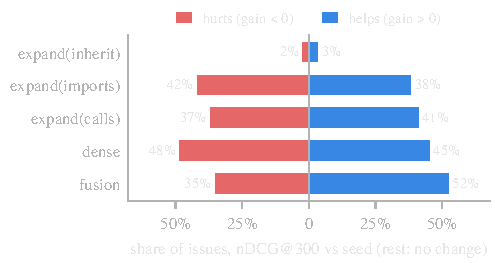
\includegraphics[height=0.55\textheight]{helps_hurts.pdf}
  \begin{itemize}
    \item Expansion helps about \textbf{40\%} of issues and hurts about \textbf{40\%}.
    \item The best action per issue would score \textbf{.258}, 40\% above fusion (.184). It is spread evenly over five actions.
  \end{itemize}
\end{frame}

\begin{frame}{Which signals predict the gain?}
  \centering
  \small
  \begin{tabular}{p{0.62\textwidth}c}
    \toprule
    Our expectation & Holds? \\
    \midrule
    Traceback $\Rightarrow$ call expansion helps & no \\
    Issue names the target file $\Rightarrow$ expansion only adds noise & no \\
    Hub top hit $\Rightarrow$ expansion floods the budget & partly \\
    BM25 and dense disagree $\Rightarrow$ use fusion & no \\
    Clear top BM25 hit $\Rightarrow$ stop & no \\
    \bottomrule
  \end{tabular}
  \vspace{6pt}
  \begin{itemize}
    \item The hub expectation holds only as a contrast: call expansion gains .017 with a weakly connected top hit and loses .014 with a hub.
    \item In a table of every feature and feature pair, about 4 times more cells show a reliable effect than chance would give. So there is signal, but it is weak.
  \end{itemize}
\end{frame}

\begin{frame}{Strongest signal: the top hit's graph degree}
  \centering
  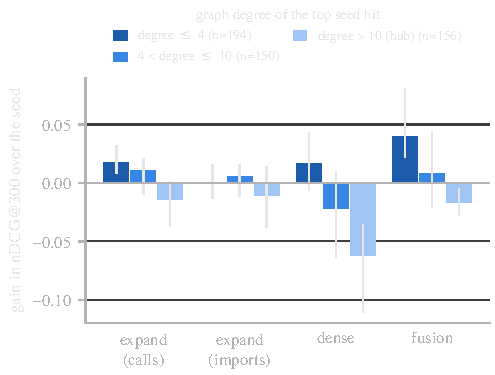
\includegraphics[height=0.6\textheight]{degree_effect.pdf}
  \begin{itemize}
    \item \textbf{Hub} top hit: dense loses .062, fusion .017. \textbf{Weakly connected}: fusion gains .040.
    \item When BM25 lands on a central definition, any change tends to hurt.
  \end{itemize}
\end{frame}

% ============================================================
\section{Phase B}

\begin{frame}{Tier 1: rules from a fixed procedure}
  \begin{itemize}
    \item Default: the best fixed action on the training issues (fusion every time).
    \item Add up to 5 rules of at most 2 conditions, greedily. Each must cover at least 20 issues from 3 repositories and show a reliably positive gain.
    \item Fit on 7 folds plus dev, tested on the held-out repository. Fixed before any held-out result.
  \end{itemize}
  \begin{block}{Rule 1, chosen in all 8 folds}
    If the top hit has \textbf{more than 7 call links} and BM25 and dense \textbf{mostly disagree}, keep the seed and \textbf{expand along calls}.\\[3pt]
    On its 64 issues: seed .202, \acn{expand(calls)} .213, fusion .161, dense .121.\\
    Dense is wrong there and fusion inherits its mistakes.
  \end{block}
\end{frame}

\begin{frame}{Results on held-out repositories}
  \centering
  \begin{tabular}{lccc}
    \toprule
    System & nDCG@300 & vs fusion & Gap closed \\
    \midrule
    \acn{stop} (BM25 seed) & .179 & & \\
    \acn{fusion} (best fixed) & .187 & & \\
    Tier 1 rules (up to 5) & .191 & $+.004$ & 5\% \\
    Tier 1, first rule only & \textbf{.193} & $+.006$ & 7\% \\
    Tier 2 classifier & .180 & $-.007$ & $-10$\% \\
    best action per issue & .262 & & \\
    \bottomrule
  \end{tabular}
  \vspace{6pt}
  \begin{itemize}
    \item 444 held-out issues. ``Gap closed'' is the share of the distance from fusion to the per-issue best that a router covers.
    \item \textbf{Neither router reliably beats fusion.} The single stable rule does best, but only barely.
  \end{itemize}
\end{frame}

\begin{frame}{Tier 2 and SWE-bench Verified}
  \centering
  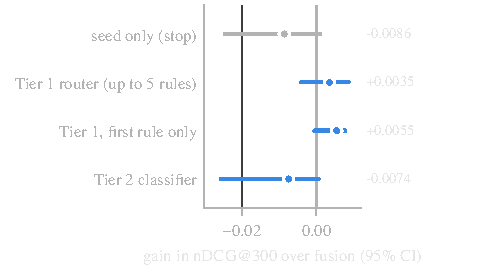
\includegraphics[height=0.47\textheight]{heldout.pdf}
  \begin{itemize}
    \item \textbf{Tier 2} (a small classifier) overfit the 56 dev issues: it moved 78\% of issues away from fusion and is reliably worse than the single rule.
    \item \textbf{SWE-bench Verified} (patched files, 464 issues): fusion .708, first rule .701, Tier 1 .690.
  \end{itemize}
\end{frame}

% ============================================================
\section{Conclusion}

\begin{frame}{What we learned}
  \begin{itemize}
    \item \textbf{The right action depends on the issue.} Expansion helps and hurts about equally often. Choosing per issue would gain 40\%.
    \item \textbf{Cheap signals predict little of it.} The strongest is how connected the top hit is. Four of our five expectations did not hold.
    \item \textbf{One rule transfers} to unseen repositories and closes about 7\% of the gap. A learned classifier does worse.
    \item \textbf{The benchmark's released nDCG} rewards a single early hit. We report the paper's definition alongside it.
    \item This is the partly negative outcome the proposal allowed for: the measurements stand, the router gain is small.
  \end{itemize}
\end{frame}

\begin{frame}{Limitations}
  \begin{itemize}
    \item Only 15 repositories, one of them 41\% of the data, so every interval is wide.
    \item The ground truth records what agents read, often whole files. It may favour broad methods like fusion over targeted expansion.
    \item Python only, one frozen dense model, one hop of expansion. We do not measure whether the agent then fixes the issue.
    \item Our Python filter wrongly dropped 41 SWE-bench Verified issues. They are covered by the Verified evaluation, not by Phase A.
    \item Tier 2 was designed after Tier 1's result was known (its own settings were fixed before its result).
  \end{itemize}
\end{frame}

\backmatter
\end{document}
